%=============================================================================
\section{Datová analytika}
%=============================================================================

\subsection{Přidaná hodnota dat pro business}

\subsubsection{Data jako strategický aktiv}

Data jsou v moderním podnikání považována za cenný aktiv -- srovnatelný s hmotným majetkem.
Přidaná hodnota dat spočívá v podpoře rozhodování na všech úrovních řízení.

\paragraph{Hierarchie dat -- DIKW pyramid}
\begin{itemize}
  \item \textbf{Data} -- nezpracovaná fakta, čísla, symboly bez kontextu
  \item \textbf{Informace} -- data s kontextem a strukturou; odpovídají na ``kdo, co, kdy, kde''
  \item \textbf{Znalost (Knowledge)} -- informace s porozuměním; odpovídá na ``jak'';
    víme \textit{jak} věci fungují a jak je využít
  \item \textbf{Moudrost (Wisdom)} -- znalost s hodnotovým soudem; odpovídá na ``proč''
\end{itemize}

\textbf{Co znamená ``znalost s hodnotovým soudem''?}
Znalost říká \textit{jak} něco udělat. Moudrost navíc říká \textit{jestli to vůbec dělat} --
přidává zkušenost, etiku a schopnost posoudit dlouhodobé důsledky. Jde o úsudek, který
nelze odvodit jen z dat, ale vyžaduje lidský kontext a hodnoty.

\textit{Příklad -- tržby firmy klesly o 30\,\%:}
\begin{center}
\begin{tabular}{p{1.6cm}p{4.2cm}p{7cm}}
\toprule
\textbf{Úroveň} & \textbf{Výrok} & \textbf{Popis} \\
\midrule
Data & ``--30\,\%, Q3 2024'' &
  Surové číslo bez vysvětlení \\
Informace & ``Tržby klesly kvůli ztrátě 3 klíčových klientů'' &
  Číslo dostalo kontext -- víme \textit{co} se stalo \\
Znalost & ``Víme, že udržení klientů vyžaduje lepší zákaznický servis a flexibilní ceny'' &
  Víme \textit{jak} problém řešit (ze zkušeností, analýz) \\
Moudrost & ``I přes krátkodobé náklady bychom měli investovat do vztahů se zákazníky -- krátkozraké snižování cen by nás poškodilo dlouhodobě'' &
  \textbf{Hodnotový soud:} rozhodnutí co je důležitější (krátkodobý zisk vs.\ dlouhodobé vztahy); vyžaduje zkušenost a etiku \\
\bottomrule
\end{tabular}
\end{center}

\textit{Jiný příklad -- lékař:} Data = teplota 38,5\,°C. Informace = pacient má horečku.
Znalost = horečka se léčí antipyretiky a klidem. Moudrost = u tohoto konkrétního staršího pacienta
se srdečním onemocněním je riziko léčby vyšší než přínos -- raději budeme monitorovat.
\textbf{Hodnotový soud} = posouzení co je v dané situaci správné, na základě zkušenosti a hodnot (primum non nocere).

\paragraph{Obchodní hodnota dat}
\begin{itemize}
  \item \textbf{Operativní rozhodování} -- automatizované, v reálném čase (fraud detection, doporučovací systémy)
  \item \textbf{Taktické rozhodování} -- střednědobé; optimalizace procesů, cen, zásob
  \item \textbf{Strategické rozhodování} -- dlouhodobé; identifikace trendů, nových trhů
  \item \textbf{Monetizace dat} -- přímý prodej dat, datové produkty (API), personalizace
\end{itemize}

\paragraph{4V dat (Big Data)}
\begin{itemize}
  \item \textbf{Volume} -- objem; terabajty až petabajty
  \item \textbf{Velocity} -- rychlost generování a zpracování
  \item \textbf{Variety} -- různorodost formátů (strukturovaná, semi-strukturovaná, nestrukturovaná)
  \item \textbf{Veracity} -- spolehlivost a přesnost dat
\end{itemize}

%=============================================================================
\subsection{Kvalita dat (Data Quality)}
%=============================================================================

\subsubsection{Dimenze kvality dat}

\textbf{Kvalita dat} je míra, do jaké data splňují požadavky pro svůj zamýšlený účel.

\begin{itemize}
  \item \textbf{Přesnost (Accuracy)} -- data odpovídají realitě (věk zákazníka je správný)
  \item \textbf{Úplnost (Completeness)} -- chybějící hodnoty (NULL, prázdné pole)
  \item \textbf{Konzistence (Consistency)} -- data jsou v souladu v rámci celého systému (stejné jméno v různých tabulkách)
  \item \textbf{Aktuálnost (Timeliness)} -- data jsou k dispozici, když jsou potřeba
  \item \textbf{Jedinečnost (Uniqueness)} -- žádné duplicitní záznamy
  \item \textbf{Validita (Validity)} -- data splňují definovaný formát a rozsah (datum ve správném formátu)
  \item \textbf{Integrita (Integrity)} -- referenční integrita zachována (FK odkazuje na existující PK)
\end{itemize}

\subsubsection{Příčiny špatné kvality dat}

\begin{itemize}
  \item Ruční zadávání dat -- překlepy, chyby
  \item Integrace více zdrojů -- různé formáty, kódování, konvence
  \item Zastaralost dat -- zákazník se přestěhoval, firma zanikla
  \item Chybějící validace na vstupu
  \item Špatně navržené databáze
\end{itemize}

\subsubsection{Data Quality Management}

Proces zajišťování a udržování kvality dat:
\begin{enumerate}
  \item \textbf{Profilování dat} -- analýza struktury, obsahu a vztahů v datech
  \item \textbf{Čištění dat (Data Cleansing)} -- oprava nebo odstranění nesprávných dat
  \item \textbf{Standardizace} -- jednotný formát (PSČ, telefonní čísla)
  \item \textbf{Deduplikace} -- odstranění duplicit (Record Linkage, fuzzy matching)
  \item \textbf{Obohacení dat} -- doplnění z externích zdrojů
  \item \textbf{Monitoring} -- průběžné sledování kvality dat (KQI -- Key Quality Indicators)
\end{enumerate}

\paragraph{Master Data Management (MDM)}
Centrální správa klíčových podnikových dat (zákazníci, produkty, zaměstnanci) -- jeden ``zlatý záznam''.

%=============================================================================
\subsection{Datový sklad, OLAP a Business Intelligence}
%=============================================================================

\subsubsection{Datový sklad (Data Warehouse)}

Centrální úložiště integrovaných dat z různých zdrojů, optimalizované pro analytické dotazy.

\textbf{Charakteristiky datového skladu (W. Inmon):}
\begin{itemize}
  \item \textbf{Subjektově orientovaný} -- data organizována kolem podnikových subjektů (zákazník, produkt), ne procesů
  \item \textbf{Integrovaný} -- data z různých zdrojů sjednocena (jednotné formáty, kódování)
  \item \textbf{Časově variantní} -- historická data; záznamy obsahují časové razítko
  \item \textbf{Neměnný (Non-volatile)} -- data se mazají jen zřídka; přidávají se nová
\end{itemize}

\paragraph{Architektura datového skladu}
\begin{itemize}
  \item \textbf{Staging area} -- dočasné uložení surových dat ze zdrojů
  \item \textbf{ETL vrstva} -- Extract, Transform, Load
  \item \textbf{Data Warehouse} -- centrální úložiště; normalizované (3NF) nebo dimenzionální schéma
  \item \textbf{Data Mart} -- podmnožina DW pro konkrétní oddělení (finance, marketing)
  \item \textbf{OLAP engine} -- analytické zpracování
  \item \textbf{Reporting/BI nástroje} -- vizualizace a reporty
\end{itemize}

\subsubsection{ETL (Extract, Transform, Load)}

\begin{enumerate}
  \item \textbf{Extract} -- extrakce dat ze zdrojových systémů (OLTP DB, CSV, ERP, CRM, API)
    \begin{itemize}
      \item Plný výběr (full load) nebo inkrementální (CDC -- Change Data Capture)
    \end{itemize}
  \item \textbf{Transform} -- transformace dat:
    \begin{itemize}
      \item Čištění (oprava chyb, NULL hodnoty)
      \item Standardizace formátů
      \item Agregace, výpočty odvozených hodnot
      \item Deduplikace
      \item Obohacení z referenčních dat
    \end{itemize}
  \item \textbf{Load} -- načtení do cílového systému
    \begin{itemize}
      \item Plné přepsání (truncate and reload)
      \item Inkrementální (pouze nová nebo změněná data)
      \item SCD (Slowly Changing Dimensions) -- správa historických změn dimenzí
    \end{itemize}
\end{enumerate}

\paragraph{ELT -- modernější alternativa}

\textbf{ELT (Extract, Load, Transform)} obrátí pořadí: data se nejprve \textit{načtou surová} do cílového
datového skladu a teprve pak se tam transformují. Transformaci provádí výpočetní výkon samotného DWH,
ne oddělený ETL server.

\begin{center}
\begin{tabular}{p{1.4cm}p{5.4cm}p{5.4cm}}
\toprule
 & \textbf{ETL} & \textbf{ELT} \\
\midrule
\textbf{Tok} &
  Zdroj $\to$ \textbf{ETL server} (transformace) $\to$ DWH &
  Zdroj $\to$ DWH raw vrstva $\to$ \textbf{DWH} (transformace) \\
\midrule
\textbf{Kde se transformuje} &
  Na dedikovaném ETL serveru (mimo DWH) &
  Přímo v DWH pomocí SQL / dbt \\
\midrule
\textbf{Raw data v DWH} &
  Ne -- načítají se až vyčištěná data &
  Ano -- raw data jsou vždy dostupná pro re-transformaci \\
\midrule
\textbf{Výkon} &
  ETL server je úzké hrdlo; škálování je drahé &
  Cloud DWH (Snowflake, BigQuery) škálují výpočty elasticky \\
\midrule
\textbf{Flexibilita} &
  Změna logiky $=$ přepsání ETL pipeline + reload &
  Změna logiky $=$ úprava SQL modelu; data jsou stále v DWH \\
\midrule
\textbf{Typické nástroje} &
  Informatica, SSIS, Talend, Pentaho &
  dbt, Fivetran + dbt, BigQuery, Snowflake \\
\midrule
\textbf{Vhodné pro} &
  On-premise; citlivá data (GDPR -- anonymizace před načtením); starší systémy &
  Cloud DWH; velké objemy; moderní datové platformy \\
\bottomrule
\end{tabular}
\end{center}

\textbf{Proč je ELT v moderním prostředí lepší:}
\begin{enumerate}
  \item \textbf{Výpočetní výkon cloudu} -- DWH jako Snowflake nebo BigQuery mají masivní paralelní
    zpracování; transformace milionů řádků trvá sekundy; ETL server by byl bottleneck
  \item \textbf{Raw data jsou vždy k dispozici} -- pokud se změní businessová logika, stačí přepsat
    transformaci a pustit ji znovu; u ETL bychom museli data znovu extrahovat ze zdrojů
  \item \textbf{Jednoduchost a verzování} -- transformace jsou čisté SQL modely; nástroj \textbf{dbt}
    (data build tool) je verzuje v Gitu, testuje a dokumentuje jako kód
  \item \textbf{Schema-on-read} -- schéma výstupních tabulek se definuje při transformaci, ne při načítání;
    snazší adaptace na změny zdrojových systémů
\end{enumerate}

\textbf{Kdy stále použít ETL:}
\begin{itemize}
  \item Citlivá data (PII, zdravotní záznamy) -- GDPR vyžaduje anonymizaci \textit{před} uložením
  \item On-premise DWH s omezenou kapacitou (nechceme ukládat surová data)
  \item Starší infrastruktura s existujícími ETL pipelines (refaktoring by byl dražší než přínos)
\end{itemize}

\subsubsection{Dimenzionální modelování}

Dimenzionální modelování (Ralph Kimball, 1990s) je přístup k návrhu datového skladu optimalizovaný
pro \textbf{analytické dotazy}. Liší se od normalizovaného relačního modelu -- záměrně připouští
redundanci výměnou za jednoduchost a rychlost čtení.

\textbf{Základní myšlenka:} každý businessový fakt (prodej, klik, platba) se dá popsat dvěma typy informací:
\begin{itemize}
  \item \textbf{Číselná měření} -- \textit{co se stalo a za kolik?} (tržba, počet kusů, marže)
  \item \textbf{Kontext} -- \textit{kdo, co, kde, kdy?} (zákazník, produkt, pobočka, datum)
\end{itemize}
Z toho vznikají dva typy tabulek: \textbf{tabulka faktů} a \textbf{dimenzionální tabulky}.

\paragraph{Tabulka faktů (Fact Table)}
Uchovává \textbf{měřitelné události} -- jeden řádek = jeden businessový fakt na dané granularitě.

\begin{itemize}
  \item Obsahuje \textbf{metriky} (číselné hodnoty k agregaci): tržba, množství, cena, marže
  \item Obsahuje pouze \textbf{cizí klíče} na dimenzionální tabulky (popis je v dimenzích, ne zde)
  \item \textbf{Granularita} -- nejdůležitější rozhodnutí návrhu: co představuje jeden řádek?
    \begin{itemize}
      \item Hrubá granularita: jeden řádek = celá objednávka (snadnější, méně řádků)
      \item Jemná granularita: jeden řádek = jedna položka na objednávce (flexibilnější, více řádků)
    \end{itemize}
\end{itemize}

\begin{center}\footnotesize
\begin{tabular}{lllllll}
\toprule
\multicolumn{7}{c}{\textbf{FAKT\_PRODEJ} (jeden řádek = jedna prodaná položka)} \\
\midrule
\underline{id\_prodeje} & id\_datum (FK) & id\_zakaznik (FK) & id\_produkt (FK) & id\_pobocka (FK) & \textbf{mnozstvi} & \textbf{trzba\_kc} \\
1 & 20240315 & 1042 & 501 & 3 & 2 & 1\,198 \\
2 & 20240315 & 1042 & 207 & 3 & 1 & 299 \\
3 & 20240316 & 871  & 501 & 1 & 1 & 599 \\
\bottomrule
\end{tabular}
\end{center}

Tučně jsou metriky (\texttt{mnozstvi}, \texttt{trzba\_kc}), vše ostatní jsou FK do dimenzí.

\paragraph{Dimenzionální tabulky (Dimension Tables)}
Poskytují \textbf{kontext a popis} k faktům. Jsou denormalizované -- záměrně obsahují redundanci,
aby se dotazy psaly jednoduše bez mnoha joinů.

\begin{center}\footnotesize
\begin{tabular}{llll}
\toprule
\multicolumn{4}{c}{\textbf{DIM\_PRODUKT}} \\
\midrule
\underline{id\_produkt} & nazev & kategorie & znacka \\
501 & Kniha Java & Knihy & O'Reilly \\
207 & Bezdrátová myš & Periferie & Logitech \\
\bottomrule
\end{tabular}
\quad
\begin{tabular}{lllll}
\toprule
\multicolumn{5}{c}{\textbf{DIM\_DATUM}} \\
\midrule
\underline{id\_datum} & datum & den\_tydne & mesic & rok \\
20240315 & 2024-03-15 & Pátek & Březen & 2024 \\
20240316 & 2024-03-16 & Sobota & Březen & 2024 \\
\bottomrule
\end{tabular}
\end{center}

Typické dimenze: \textbf{Čas} (den/týden/měsíc/rok/čtvrtletí), \textbf{Zákazník} (jméno/segment/region),
\textbf{Produkt} (název/kategorie/značka), \textbf{Pobočka/Lokalita} (město/kraj/země).

\paragraph{Hvězdicové schéma (Star Schema)}
Centrální tabulka faktů je obklopena dimenzionálními tabulkami -- vizuálně připomíná hvězdu.
Dimenze \textbf{nejsou normalizovány} (obsahují redundanci).

\begin{figure}[H]
\centering
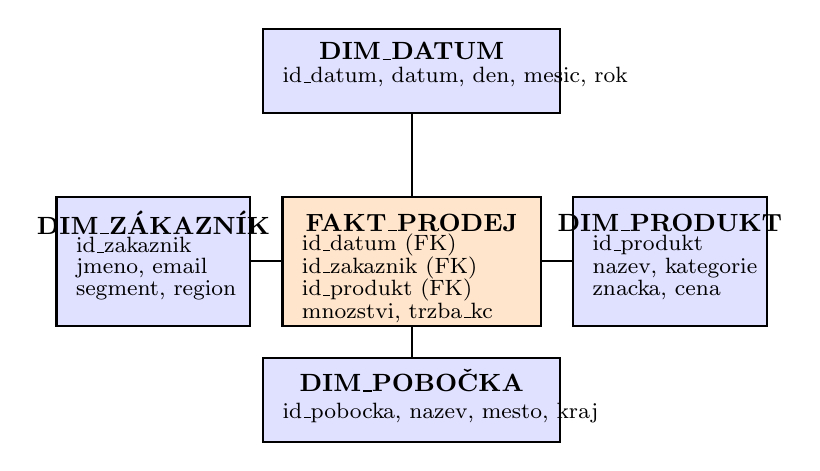
\begin{tikzpicture}[font=\footnotesize, scale=0.82]
  % Central fact table
  \draw[fill=orange!20, thick] (3.5,2.2) rectangle (7.5,4.2);
  \node[font=\small\bfseries] at (5.5,3.8) {FAKT\_PRODEJ};
  \node[anchor=west] at (3.65,3.45) {id\_datum (FK)};
  \node[anchor=west] at (3.65,3.1) {id\_zakaznik (FK)};
  \node[anchor=west] at (3.65,2.75) {id\_produkt (FK)};
  \node[anchor=west] at (3.65,2.4) {mnozstvi, trzba\_kc};
  % DIM_DATUM (top)
  \draw[fill=blue!12, thick] (3.2,5.5) rectangle (7.8,6.8);
  \node[font=\small\bfseries] at (5.5,6.45) {DIM\_DATUM};
  \node[anchor=west] at (3.35,6.05) {id\_datum, datum, den, mesic, rok};
  % DIM_ZAKAZNIK (left)
  \draw[fill=blue!12, thick] (0,2.2) rectangle (3.0,4.2);
  \node[font=\small\bfseries] at (1.5,3.8) {DIM\_ZÁKAZNÍK};
  \node[anchor=west] at (0.15,3.45) {id\_zakaznik};
  \node[anchor=west] at (0.15,3.1) {jmeno, email};
  \node[anchor=west] at (0.15,2.75) {segment, region};
  % DIM_PRODUKT (right)
  \draw[fill=blue!12, thick] (8.0,2.2) rectangle (11.0,4.2);
  \node[font=\small\bfseries] at (9.5,3.8) {DIM\_PRODUKT};
  \node[anchor=west] at (8.15,3.45) {id\_produkt};
  \node[anchor=west] at (8.15,3.1) {nazev, kategorie};
  \node[anchor=west] at (8.15,2.75) {znacka, cena};
  % DIM_POBOCKA (bottom)
  \draw[fill=blue!12, thick] (3.2,0.4) rectangle (7.8,1.7);
  \node[font=\small\bfseries] at (5.5,1.35) {DIM\_POBOČKA};
  \node[anchor=west] at (3.35,0.85) {id\_pobocka, nazev, mesto, kraj};
  % Connecting lines
  \draw[thick] (5.5,4.2) -- (5.5,5.5);
  \draw[thick] (3.5,3.2) -- (3.0,3.2);
  \draw[thick] (7.5,3.2) -- (8.0,3.2);
  \draw[thick] (5.5,2.2) -- (5.5,1.7);
\end{tikzpicture}
\caption{Hvězdicové schéma (Star Schema) -- e-shop prodeje}
\label{fig:star}
\end{figure}

\textbf{Výhody:} jednoduché dotazy (málo joinů), rychlé čtení, srozumitelné pro business uživatele.
\textbf{Nevýhody:} redundance v dimenzích (jméno zákazníka se opakuje).

\paragraph{Sněhové schéma (Snowflake Schema)}
Dimenzionální tabulky jsou \textbf{normalizovány} -- kategorie produktu je v samostatné tabulce,
kraj zákazníka v jiné. Vizuálně připomíná sněhovou vločku.

\textbf{Výhody:} méně redundance, menší objem dat.
\textbf{Nevýhody:} více joinů = pomalejší dotazy; složitější pro analytiky.

\textit{V praxi se používá hvězdicové schéma -- rychlost dotazů je důležitější než úspora místa.}

\paragraph{Příklad analytického dotazu nad hvězdicovým schématem}
\begin{lstlisting}[language=SQL, caption=Tržby podle kategorie a měsíce -- typický DWH dotaz]
SELECT  p.kategorie,
        d.mesic,
        d.rok,
        SUM(f.trzba_kc)   AS celkova_trzba,
        COUNT(*)          AS pocet_prodanu
FROM    FAKT_PRODEJ f
JOIN    DIM_PRODUKT p  ON f.id_produkt  = p.id_produkt
JOIN    DIM_DATUM   d  ON f.id_datum    = d.id_datum
WHERE   d.rok = 2024
GROUP BY p.kategorie, d.mesic, d.rok
ORDER BY d.mesic, celkova_trzba DESC;
\end{lstlisting}

\subsubsection{OLAP (Online Analytical Processing)}

OLAP umožňuje interaktivní analýzu dat z více perspektiv (dimenzí).

\paragraph{OLAP operace}
\begin{itemize}
  \item \textbf{Drill-down} -- přechod na nižší úroveň granularity (rok $\to$ čtvrtletí $\to$ měsíc)
  \item \textbf{Roll-up (Drill-up)} -- agregace na vyšší úroveň (měsíc $\to$ rok)
  \item \textbf{Slice} -- výběr jedné dimenze (prodeje pouze pro rok 2023)
  \item \textbf{Dice} -- výběr podkubu (prodeje pro rok 2023 a region CZ)
  \item \textbf{Pivot (Rotate)} -- rotace pohledu na data
\end{itemize}

\paragraph{Typy OLAP}
\begin{itemize}
  \item \textbf{MOLAP} -- multidimenzionální; data v speciálních kubech; rychlé, ale omezená škálovatelnost
  \item \textbf{ROLAP} -- relační; nad standardním DWH; škálovatelné, flexibilní
  \item \textbf{HOLAP} -- hybridní; kombinuje MOLAP a ROLAP
\end{itemize}

\subsubsection{KPI, Dimenze, Granularita}

\begin{itemize}
  \item \textbf{KPI (Key Performance Indicators)} -- klíčové ukazatele výkonnosti; měřitelné hodnoty
    hodnotící výkonnost organizace vůči cílům
    \begin{itemize}
      \item Příklady: konverzní poměr, průměrná hodnota objednávky, NPS, churn rate
      \item Musí být SMART: Specific, Measurable, Achievable, Relevant, Time-bound
    \end{itemize}
  \item \textbf{Dimenze} -- perspektiva, z níž se data analyzují (čas, zákazník, produkt, lokalita)
  \item \textbf{Granularita} -- úroveň detailu dat; jemnější granularita = více prostoru, více flexibility
  \item \textbf{Agregace} -- shrnutí dat (SUM, AVG, COUNT, MIN, MAX) na vyšší úroveň granularity
  \item \textbf{Metrika/Míra} -- numerická hodnota podléhající agregaci (obrat, počet kusů)
\end{itemize}

\subsubsection{Business Intelligence (BI)}

\textbf{BI} je soubor technologií, procesů a nástrojů pro transformaci surových dat na srozumitelné,
použitelné informace pro obchodní rozhodování.

\paragraph{Složky BI}
\begin{itemize}
  \item Datový sklad + ETL/ELT pipeline
  \item OLAP engine
  \item Reporting a dashboardy
  \item Data mining a prediktivní analytika
  \item Self-service BI (Power BI, Tableau, Qlik)
\end{itemize}

\paragraph{Praktický příklad: analýza zákazníků z MSSQL pomocí BI}

Máš transakční databázi v MS SQL Serveru s tabulkami zákazníků a objednávek.
Cíl: pochopit chování zákazníků, odhalit trendy, podpořit rozhodování.
Celý tok od zdrojové DB po dashboard vypadá takto:

\medskip
\textbf{Krok 1 -- Zdrojová data (OLTP databáze v MSSQL)}

Transakční DB je navržena pro rychlé zápisy, ne pro analytiku. Dotaz jako
``měsíční tržby podle segmentu zákazníka za posledních 5 let'' by blokoval produkční server.

\begin{lstlisting}[language=SQL, caption=Zdrojové tabulky v MSSQL (OLTP)]
-- Tabulky existující v produkčním MSSQL
SELECT TOP 5 * FROM Customers;   -- id, name, email, segment, region, created_at
SELECT TOP 5 * FROM Orders;      -- id, customer_id, order_date, total_amount, status
SELECT TOP 5 * FROM OrderItems;  -- id, order_id, product_id, qty, unit_price
\end{lstlisting}

\textbf{Krok 2 -- ETL/ELT: přesun dat do datového skladu}

Produkční data se pravidelně (nočně nebo v reálném čase) přesouvají do DWH
a transformují do hvězdicového schématu:

\begin{lstlisting}[language=SQL, caption=Dimenzionální model v DWH (hvězdicové schéma)]
-- DWH tabulky (Power BI / Azure Synapse / SQL Server DW)
DIM_ZAKAZNIK (id_zak, jmeno, segment, region, datum_registrace)
DIM_CAS      (id_cas, datum, mesic, kvartal, rok, den_tydne)
DIM_PRODUKT  (id_prod, nazev, kategorie, znacka)
FAKT_PRODEJ  (id_zak_fk, id_cas_fk, id_prod_fk, trzba, mnozstvi, sleva)
\end{lstlisting}

\textbf{Krok 3 -- Připojení Power BI k datům}

Power BI se připojí přímo k MSSQL nebo k DWH přes konektor.
V Power BI Desktop: \textit{Získat data} $\to$ \textit{SQL Server} $\to$ zadáš server a DB.
Power BI automaticky detekuje relace mezi tabulkami (FK).

\textbf{Krok 4 -- Výpočty v Power BI pomocí DAX}

DAX (Data Analysis Expressions) je jazyk Power BI pro metriky:

\begin{lstlisting}[language=SQL, caption=DAX výpočty v Power BI]
-- Celková tržba
Celkova trzba = SUM(FAKT_PRODEJ[trzba])

-- Tržba za předchozí rok (pro porovnání)
Trzba loni = CALCULATE([Celkova trzba], SAMEPERIODLASTYEAR(DIM_CAS[datum]))

-- Meziroční růst v %
Rust YoY % = DIVIDE([Celkova trzba] - [Trzba loni], [Trzba loni]) * 100

-- Počet aktivních zákazníků (alespoň 1 nákup za posledních 90 dní)
Aktivni zakaznici =
    CALCULATE(
        DISTINCTCOUNT(FAKT_PRODEJ[id_zak_fk]),
        DATESINPERIOD(DIM_CAS[datum], TODAY(), -90, DAY)
    )
\end{lstlisting}

\textbf{Krok 5 -- Vizualizace a dashboard}

V Power BI sestavíš dashboard z vizuálů:

\begin{center}
\begin{tabular}{p{3.5cm}p{4cm}p{5cm}}
\toprule
\textbf{Vizuál} & \textbf{Co zobrazuje} & \textbf{Businessová otázka} \\
\midrule
Sloupcový graf & Tržby podle měsíce + loni & Rosteme nebo klesáme YoY? \\
Mapa & Tržby podle regionu & Kde jsou naši nejcennější zákazníci? \\
Koláčový/pruhový & Podíl segmentů (Premium/Standard/Budget) & Který segment nás živí? \\
KPI karta & Celková tržba, aktivní zákazníci, průměrná objednávka & Rychlý přehled klíčových čísel \\
Tabulka & Top 10 zákazníků (RFM analýza) & Na koho se zaměřit? \\
Průběhový graf & Churn rate (\% zákazníků bez nákupu 6 měsíců) & Přicházíme o zákazníky? \\
\bottomrule
\end{tabular}
\end{center}

\textbf{Krok 6 -- Filtry (Slicery) a drill-through}

Uživatel si může dashboard sám filtrovat:
\begin{itemize}
  \item \textbf{Slicer} -- filtr na období (rok/čtvrtletí), region, segment zákazníka
  \item \textbf{Drill-through} -- klik na region na mapě $\to$ přejde na detailní stránku tohoto regionu
  \item \textbf{Cross-filtering} -- klik na sloupec v grafu automaticky filtruje všechny ostatní vizuály
\end{itemize}

\textbf{Publikace a sdílení} -- hotový report se publikuje do Power BI Service (cloud);
manažeři ho vidí v prohlížeči nebo mobilní aplikaci; reporty se mohou automaticky aktualizovat.

\medskip
\textbf{Celkový tok od dat k rozhodnutí:}

\begin{center}
\small
MSSQL (zákazníci, objednávky) $\xrightarrow{\text{ETL/ELT}}$
Datový sklad (hvězda) $\xrightarrow{\text{Power BI konektor}}$
DAX metriky $\xrightarrow{\text{vizualizace}}$
Dashboard $\xrightarrow{\text{publish}}$
Manažerské rozhodování
\end{center}

\subsubsection{Balanced Scorecard (BSC)}

\textbf{BSC} (Kaplan \& Norton, 1992) je strategický nástroj pro měření a řízení výkonnosti organizace
z více perspektiv -- překlenuje propast mezi strategií a operativou.

\paragraph{4 perspektivy BSC}
\begin{itemize}
  \item \textbf{Finanční perspektiva} -- jak nás vnímají akcionáři? KPI: ROI, ROE, zisk, náklady
  \item \textbf{Zákaznická perspektiva} -- jak nás vnímají zákazníci? KPI: spokojenost, NPS, retence, podíl na trhu
  \item \textbf{Perspektiva interních procesů} -- v čem musíme excelovat? KPI: čas cyklu, kvalita, inovace
  \item \textbf{Perspektiva učení a růstu} -- jak rozvíjíme schopnosti? KPI: školení, fluktuace, spokojenost zaměstnanců
\end{itemize}

Každá perspektiva obsahuje: strategický záměr $\to$ cíle $\to$ metriky $\to$ iniciativy.
BSC propojuje KPI s firemní strategií -- nestačí sledovat jen finanční ukazatele.

\begin{profesorbox}[Otázky profesorů k tématu: Datová analytika]
\textbf{Pour Jan, doc. Ing., CSc.}
\begin{itemize}
  \item Co je datový sklad a jaké jsou jeho charakteristiky?
  \item Jaký je rozdíl mezi OLTP a OLAP?
  \item Co je ETL a jaké jsou jeho fáze?
\end{itemize}
\textbf{Maryška Miloš, doc. Ing., Ph.D.}
\begin{itemize}
  \item Jaké jsou dimenze kvality dat?
  \item Co je KPI a jak se definuje?
  \item Vysvětlete pojem granularita v kontextu datového skladu.
\end{itemize}
\textbf{Sudzina František, Mgr.\ et Mgr.\ Ing., Ph.D.}
\begin{itemize}
  \item Jaká jsou V velkých dat (Big Data)?
  \item Co je Business Intelligence a jaké nástroje znáte?
\end{itemize}
\textbf{Chudán David, Ing., Ph.D.}
\begin{itemize}
  \item Jaké jsou OLAP operace? Vysvětlete drill-down a roll-up.
  \item Co je hvězdicové a sněhové schéma?
\end{itemize}
\end{profesorbox}
